\documentclass[tikz,border=4pt]{standalone}
\usepackage[T1]{fontenc}
\usepackage{lmodern}
\usetikzlibrary{positioning,arrows.meta,fit,backgrounds,calc}
% One colour dimension: which level a check works at.
%   cool (teal) = verification, per claim; warm (amber) = validation, once; gray = structure.
\definecolor{ver}{HTML}{1F7A7A}
\definecolor{verbg}{HTML}{E6F2F2}
\definecolor{val}{HTML}{B5651D}
\definecolor{valbg}{HTML}{FBEEDD}
\definecolor{struct}{HTML}{555555}
\begin{document}
\sffamily\footnotesize
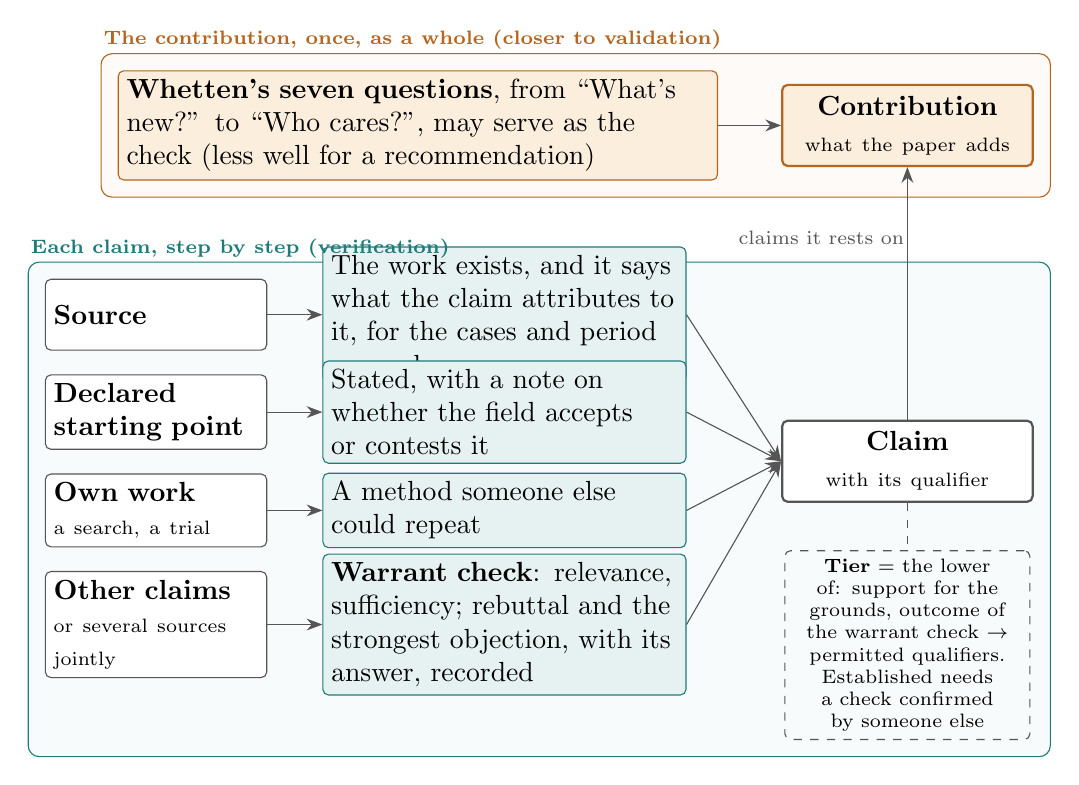
\begin{tikzpicture}[
  node distance=3mm and 7mm,
  every node/.append style={execute at begin node={\hyphenpenalty=10000 \exhyphenpenalty=10000 }},
  ground/.style={draw=struct, rounded corners=2pt, text width=2.6cm, minimum height=9mm, align=left, inner sep=3pt, fill=white},
  check/.style={draw=ver, rounded corners=2pt, text width=4.4cm, minimum height=9mm, align=left, inner sep=3pt, fill=verbg},
  claim/.style={draw=struct, thick, rounded corners=2pt, text width=2.9cm, align=center, inner sep=4pt, fill=white},
  arr/.style={-{Stealth[length=2mm]}, struct},
  band/.style={font=\scriptsize\bfseries, anchor=south west, inner sep=1pt},
]
% --- Verification band: one claim, its grounds item by item ---
\node[ground] (src) {\textbf{Source}};
\node[ground, below=of src] (decl) {\textbf{Declared starting point}};
\node[ground, below=of decl] (own) {\textbf{Own work}\\ \scriptsize a search, a trial};
\node[ground, below=of own] (oth) {\textbf{Other claims}\\ \scriptsize or several sources jointly};

\node[check, right=of src] (csrc) {The work exists, and it says what the claim attributes to it, for the cases and period covered};
\node[check, right=of decl] (cdecl) {Stated, with a note on whether the field accepts or contests it};
\node[check, right=of own] (cown) {A method someone else could repeat};
\node[check, right=of oth] (coth) {\textbf{Warrant check}: relevance, sufficiency; rebuttal and the strongest objection, with its answer, recorded};

\foreach \g/\c in {src/csrc, decl/cdecl, own/cown, oth/coth} \draw[arr] (\g) -- (\c);

\node[claim, right=12mm of $(cdecl.east)!0.5!(cown.east)$] (claim) {\textbf{Claim}\\[1pt] \scriptsize with its qualifier};
\foreach \c in {csrc, cdecl, cown, coth} \draw[arr] (\c.east) -- (claim.west);

\node[draw=struct, dashed, rounded corners=2pt, text width=2.9cm, align=center, inner sep=3pt, below=6mm of claim, font=\scriptsize] (tier)
  {\textbf{Tier} = the lower of: support for the grounds, outcome of the warrant check $\rightarrow$ permitted qualifiers. Established needs a check confirmed by someone else};
\draw[struct, dashed] (claim) -- (tier);

\begin{scope}[on background layer]
  \node[fit=(src)(oth)(coth)(claim)(tier), draw=ver, rounded corners=4pt, inner sep=6pt, fill=ver!3] (verband) {};
\end{scope}
\node[band, text=ver] at (verband.north west) {Each claim, step by step (verification)};

% --- Validation band: the contribution, once ---
\node[claim, fill=valbg, draw=val, anchor=south] (contr) at ($(verband.north -| claim)+(0,12mm)$) {\textbf{Contribution}\\[1pt] \scriptsize what the paper adds};
\node[draw=val, rounded corners=2pt, text width=7.4cm, align=left, inner sep=3pt, fill=valbg, left=8mm of contr] (whet)
  {\textbf{Whetten's seven questions}, from ``What's new?'' to ``Who cares?'', may serve as the check (less well for a recommendation)};
\draw[arr] (whet) -- (contr);
\draw[arr] (claim.north) -- node[pos=0.72, left, font=\scriptsize, text=struct, fill=white, inner sep=1pt] {claims it rests on} (contr.south);

\begin{scope}[on background layer]
  \node[fit=(whet)(contr), draw=val, rounded corners=4pt, inner sep=6pt, fill=val!3] (valband) {};
\end{scope}
\node[band, text=val] at (valband.north west) {The contribution, once, as a whole (closer to validation)};
\end{tikzpicture}
\end{document}
